\documentclass
[
a4paper,															% Papierformat
12pt,																% Schriftgröße
twoside=true,														% Zweiseitig
openright,															% Neues Kapitel immer auf der rechten Seite
titlepage,															% Titelseite
headinclude,														% Seitengröße auch bei Kopfzeile
numbers=noenddot,													% Bei Kapiteln keine abschließenden Punkte
listof=numbered,													% Listingsverzeichnis
bibliography=totocnumbered,											% Literaturverzeichnis
]
{scrbook}															% Dokumenttyp

\usepackage[bottom=1in,inner=1in,outer=20mm,top=20mm]{geometry}		% Ganze Seite verwenden

% Kopf und Fußzeile
\usepackage{emptypage}												% Leere Seiten ohne Kopf und Fußzeile
\usepackage[headsepline]{scrlayer-scrpage}							% Kopf und Fußzeile
\pagestyle{scrheadings}												% Nummerierung in der Kopfzeile
\clearscrheadfoot													% Kopf und Fußzeile löschen
\rehead{\headmark}													% Kapitelname auf der geraden Seite innen
\ohead[\pagemark]{\pagemark}										% Seitennummerierung
\lohead{}															% Name auf der ungeraden Seite innen
\renewcommand*{\chapterpagestyle}{scrheadings}						% Kopf und Fußzeile auf Seiten mit Überschriften anders

% Dokumenteinstellungen und Paketimporte
\usepackage[T1]{fontenc}											% Outputencoding
\usepackage{lmodern}
\usepackage[utf8]{inputenc}											% UTF8 + Sonderzeichen
\usepackage{newtxtext, newtxmath}									% Font Verbesserungen (z.B. µ direkt verwendbar)
\usepackage[ngerman]{babel}											% Deutsch
\usepackage{caption}												% Tabellen Listings und Figuren mit Beschriftung in Verzeichnissen
\usepackage[hyphens]{url}											% Zeilenumbruch bei URLs
\usepackage{graphicx}												% Bilder
\usepackage{float}													% Plazierung von Floats (Bilder Tabellen)
\usepackage{wrapfig}												% Textumfluss von Bildern, die nicht die ganze Seite brauchen
\usepackage{setspace}												% Zeilenabstand
\usepackage{listings}												% Listings (=Code)
\usepackage{courier}												% Courier (listings)
\usepackage{times}													% Schriftart Times Roman
\usepackage{courier}												% Schriftart Courier
\usepackage{array,multirow}											% Bessere Tabellenformatierung
\usepackage{xcolor}													% Farben für Codehighlighting oder ähnliches
\usepackage{tabularx}												% Bessere Tabellen
\usepackage{appendix}												% Anhang Titelseite
\usepackage[printonlyused,withpage]{acronym}						% Für die Verwendung von Akronymen + Verzeichnis - printonlyused: Abkürzung nur im Verzeichnis wenn auch benutzt; withpage: Seite der 1. Verwendung im Verzeichnis anzeigen

\setlength{\parindent}{0em}											% Einrücken
\setcounter{tocdepth}{5}											% Tiefe der Überschriften
\setcounter{secnumdepth}{5}											% Nummerierungstiefe der Überschriften

%Style for the \inlinecode{}{} command
%command use: \inlinecode{language}{code} e.g.: \inlinecode{Java}{public static void main()}
\lstset{
backgroundcolor=\color{codeBackGray},
showstringspaces=false,
keepspaces=true,
basicstyle=\footnotesize\ttfamily,
keywordstyle=\color{blue},
commentstyle=\color[grey]{0.6},
stringstyle=\color[RGB]{255,150,75}
}

%Hier soll die bei dem int-Array kein Zeilenumbruch stattfinden (Formatierung ganz ausschalten???)
%Java
%Model from netbeans
\definecolor{java_net_comment}{rgb}{0.586,0.586,0.586}
\definecolor{java_net_keyword}{rgb}{0,0,0.898}
\definecolor{java_net_string}{rgb}{0.805,0.480,0}
\definecolor{java_net_preprocessor}{rgb}{0,0.597,0}
\definecolor{codeBackGray}{gray}{0.98}

\lstdefinestyle{java}{ 																					% define java style
language=Java,                 																		% the language of the code
backgroundcolor=\color{codeBackGray},   																% choose the background color
basicstyle=\footnotesize\ttfamily,,																	% the size and the font that are used for the code
breakatwhitespace=false,         																		% sets if automatic breaks should only happen at whitespace
breaklines=true,                 																		% sets automatic line breaking
captionpos=b,                    																		% sets the caption-position to bottom
xleftmargin={0.75cm},																				    % align code with text
commentstyle=\color{java_net_comment},    															% comment style
escapeinside={(*}{*)},          																		% if you want to add LaTeX within your code
extendedchars=true,             		 																% lets you use non-ASCII characters; for 8-bits encodings only, does not work with UTF-8
frame=none,%single,	                   																% adds a frame around the code
framexleftmargin=8mm,																					% include numbers into the frame
keepspaces=true,                																		% keeps spaces in text, useful for keeping indentation of code (possibly needs columns=flexible)
keywordstyle=\color{java_net_keyword},       															% keyword style
deletekeywords=          																				% if you want to delete keywords from the given language
{},
otherkeywords={},           																			% if you want to add more keywords to the set
numbers=left,                    																		% where to put the line-numbers; possible values are (none, left, right)
numbersep=8pt,                   																		% how far the line-numbers are from the code
numberstyle=\footnotesize\ttfamily,																	% the style that is used for the line-numbers
rulecolor=\color{black},         																		% if not set, the frame-color may be changed on line-breaks within not-black text (e.g. comments (green here))
showspaces=false,                																		% show spaces everywhere adding particular underscores; it overrides 'showstringspaces'
showstringspaces=false,          																		% underline spaces within strings only
showtabs=false,                  																		% show tabs within strings adding particular underscores
stepnumber=1,                    																		% the step between two line-numbers. If it's 1, each line will be numbered
stringstyle=\color{java_net_string},     																% string literal style
tabsize=2,	                   																		% sets default tabsize to 2 spaces
title=\lstname,                  		 																% show the filename of files included with
literate=%
{_}{{\_}}1
{Ö}{{\"O}}1
{Ä}{{\"A}}1
{Ü}{{\"U}}1
{ß}{{\ss}}1
{ü}{{\"u}}1
{ä}{{\"a}}1
{ö}{{\"o}}1																							% escape ÖÄÜßüäö
}
%C
%Model from netbeans
\definecolor{C_net_comment}{rgb}{0.586,0.586,0.586}
\definecolor{C_net_keyword}{rgb}{0,0,0.898}
\definecolor{C_net_string}{rgb}{0.805,0.480,0}
\definecolor{C_net_preprocessor}{rgb}{0,0.597,0}
\definecolor{codeBackGray}{gray}{0.98}

\lstdefinestyle{C}{ 																					% define c style
language=C,                 																			% the language of the code
backgroundcolor=\color{codeBackGray},   																% choose the background color; you must add \usepackage{color} or \usepackage{xcolor}
basicstyle=\footnotesize\ttfamily,													        		% the size of the fonts that are used for the code
breakatwhitespace=false,         																		% sets if automatic breaks should only happen at whitespace
breaklines=true,                 																		% sets automatic line breaking
captionpos=b,                    																		% sets the caption-position to bottom
xleftmargin={0.75cm},																					% align code with text
commentstyle=\color{C_net_comment},    																% comment style
escapeinside={(*}{*)},          																		% if you want to add LaTeX within your code
extendedchars=true,             		 																% lets you use non-ASCII characters; for 8-bits encodings only, does not work with UTF-8
frame=none,%single,	                   																% adds a frame around the code
framexleftmargin=8mm,																					% include numbers into the frame
keepspaces=true,                																		% keeps spaces in text, useful for keeping indentation of code (possibly needs columns=flexible)
keywordstyle=\color{C_net_keyword},       															% keyword style
deletekeywords=          																				% if you want to delete keywords from the given language
{...},
otherkeywords={*,...},           																		% if you want to add more keywords to the set
numbers=left,                    																		% where to put the line-numbers; possible values are (none, left, right)
numbersep=8pt,                   																		% how far the line-numbers are from the code
numberstyle=\footnotesize\ttfamily,																	% the style that is used for the line-numbers
rulecolor=\color{black},         																		% if not set, the frame-color may be changed on line-breaks within not-black text (e.g. comments (green here))
showspaces=false,                																		% show spaces everywhere adding particular underscores; it overrides 'showstringspaces'
showstringspaces=false,          																		% underline spaces within strings only
showtabs=false,                  																		% show tabs within strings adding particular underscores
stepnumber=1,                    																		% the step between two line-numbers. If it's 1, each line will be numbered
stringstyle=\color{C_net_string},     																% string literal style
tabsize=2,	                   																		% sets default tabsize to 2 spaces
title=\lstname,                  		 																% show the filename of files included with
literate=
{\#include}{{{\color{C_net_preprocessor}\#include}}}{8}
{\#define}{{{\color{C_net_preprocessor}\#define}}}{7}
{_}{{\_}}1
{Ö}{{\"O}}1
{Ä}{{\"A}}1
{Ü}{{\"U}}1
{ß}{{\ss}}1
{ü}{{\"u}}1
{ä}{{\"a}}1
{ö}{{\"o}}1																							% escape ÖÄÜßüäö
}
\definecolor{editorGray}{cmyk}{0, 0, 0, 0.2}
\newcommand{\inlinecode}[2]{\colorbox{editorGray}{\lstinline[style=#1]$#2$}}

\expandafter\def\expandafter\UrlBreaks\expandafter{\UrlBreaks% save the current one
\do\a\do\b\do\c\do\d\do\e\do\f\do\g\do\h\do\i\do\j%
\do\k\do\l\do\m\do\n\do\o\do\p\do\q\do\r\do\s\do\t%
\do\u\do\v\do\w\do\x\do\y\do\z\do\A\do\B\do\C\do\D%
\do\E\do\F\do\G\do\H\do\I\do\J\do\K\do\L\do\M\do\N%
\do\O\do\P\do\Q\do\R\do\S\do\T\do\U\do\V\do\W\do\X%
\do\Y\do\Z\do\*\do\-\do\~\do\'\do\"\do\-}%													% Datei importieren
\usepackage[autostyle]{csquotes}
\usepackage[
    backend=biber,
    style=apa,
    sortlocale=de_DE,
    isbn=true
]{biblatex}
\addbibresource{Literaturverzeichnis.bib}
\setlength{\bibitemsep}{1em}
\setcounter{biburllcpenalty}{7000}
\setcounter{biburlucpenalty}{8000}
\DeclareLabeldate{
    \field{date}
    \field{eventdate}
    \field{origdate}
}

\usepackage[bookmarks]{hyperref}									% Automatische Lesezeichen
\usepackage[figure]{hypcap} 										% Bild referenzieren

\subject{\includegraphics[scale=0.7]{fig/logoMecha}}
\title{Diplomarbeitvorlage}
\subtitle{HTBLA Kaindorf an der Sulm\\
Grazer Straße 202, A-8430 Kaindorf an der Sulm\\
Ausbildungsschwerpunkt Mechatronik und Automatisierungstechnik}
\author{Florian Greistorfer \and Marian Korošec}
\date{Abgabedatum: 7.3.2018}
\publishers{Betreut von:\\Dipl.-Ing. Manfred Steiner}
\begin{document}													% Dokumentbeginn
\onehalfspace														% Zeilenabstand
\maketitle															% Titelseite
\frontmatter												%Seitennumerierung
\pagenumbering{Roman}										%Römische Zahlen
\addtocounter{page}{2}

\newcommand{\doublesignature}[2]{%
  \parbox{\textwidth}{
    \hfill
    \parbox{7cm}{
      \centering
      \rule{6cm}{1pt}\\
      #1
    }
    \parbox{7cm}{
      \centering
      \rule{6cm}{1pt}\\
      #2
    }
  }
  \mbox{}\\
  \mbox{}\\
  \mbox{}\\
  \mbox{}\\
}

\vspace*{20pt}

\section*{Eidesstattliche Erklärung}
\label{sec:eidesstattliche-erklaerung}
Ich erkläre an Eides statt, dass ich die vorliegende Arbeit selbstständig verfasst, andere als die angegebenen
Quellen/Hilfsmittel nicht benutzt und die den benutzten Quellen wörtlich und inhaltlich entnommenen
Stellen als solche kenntlich gemacht habe.\\
\\
Arnfels, am 5. April 2018\\

\vskip 1cm

\doublesignature{Stefan Hörmann}{Nicolas Perl}
\doublesignature{Alois Vollmaier}{Mr. Mösensaft}

\vskip 5cm

\clearpage

\newpage
\thispagestyle{empty}
\mbox{}

\clearpage

\section*{Danksagung}
\label{sec:danksagung}
An dieser Stelle möchten wir uns bei allen bedanken, die uns im Rahmen der Diplomarbeit unterstützt und betreut haben.\\
\\
TODO

\clearpage

\newpage
\thispagestyle{empty}
\mbox{}

\clearpage

\section*{Abstract}
\label{sec:abstract}
TODO

\section*{Zusammenfassung}
Wir setzten uns als Ziel eine Maschine zu entwickeln, welche das Mischen, sowie das Ausgeben von Spielkarten übernimmt.
Die Idee ist es, diese Verfahren möglichst platzsparend, zeiteffizient und detailliert durchdacht und optimiert zu realisieren.\\


\begin{figure}[H]
  \centering
  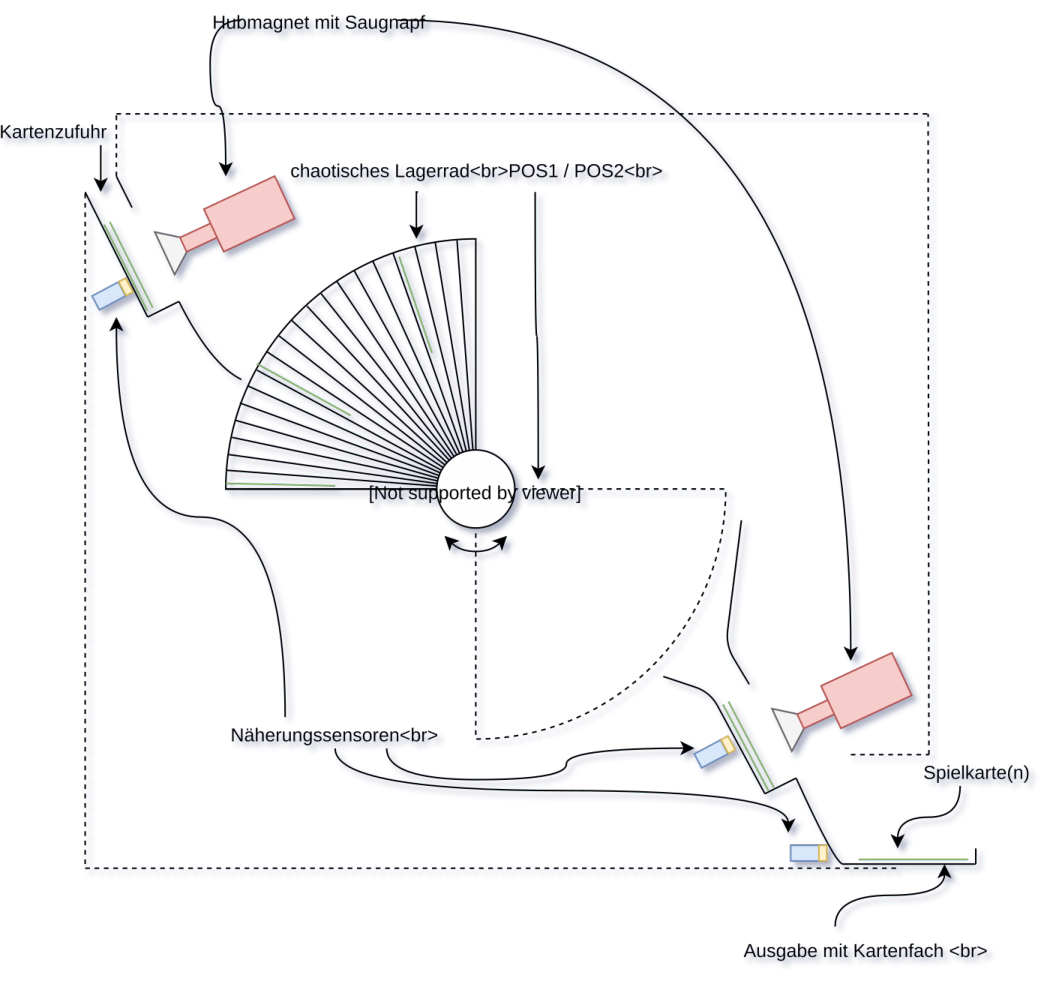
\includegraphics[width=0.6\textwidth]{fig/Reshuffled_Version_3_0_prinzip.pdf}
  \caption{Name des Bildes}
  \label{fig:verweis}
\end{figure}

Grundsätzlich basiert das Mischprinzip auf einer Art "Fächersystem".
Eingelegte Karten gelangen mithilfe eines ausgeklügelten Systems, welches aus einem Hubmagneten mit integriertem Saugnapf besteht, aus dem Einlegefach.
Erfolgt die Kartenentnahme, rutscht die Karte in ein zufälliges Fach des Lagerrads. Anschließend wird dieses Lagerrad in Drehbewegung versetzt um die gelagerten Karten auszugeben.

Der Benutzer steuert diese Maschiene mithilfe einer GUI welche auf einem 7" LCD Display angezeigt wird. Systemintern steuert ein 8-Bit Mikrocontroller der AVR-Familie den Ablauf.

\clearpage

\newpage
\thispagestyle{empty}
\mbox{}

\clearpage

\subsection*{Gender Erklärung}
\label{sec:gender-erklaerung}
Aus Gründen der besseren Lesbarkeit wird in dieser Arbeit die Sprachform des generischen Maskulinums angewendet. Es wird an dieser Stelle darauf hingewiesen, dass die ausschließliche Verwendung der männlichen Form geschlechtsunabhängig verstanden werden soll.

\subsection*{Über dieses Dokument}
\label{sec:ueber-dokument}
Diese Arbeit wurde in \LaTeX{} verfasst. Diese Art der Dokumentation bietet gegenüber den normalen Textverarbeitungen gewisse Vorteile hinsichtlich der Formatierung und des Einbindens von Grafiken. Auch Formeln können sehr einfach und effizient angegegeben werden. Die Rohfassung des Dokuments befindet sich auf dem Arnfelser Gitweb Server der HTBLA Kaindorf Abteilung Mechatronik.

\clearpage

\newpage
\thispagestyle{empty}
\mbox{}

\clearpage

\section*{Projektteam}
\label{sec:projektteam}

\subsection*{Stefan Hörmann}
\begin{wrapfigure}[10]{l}{0.5\textwidth}
\begin{center}
  \includegraphics[width=0.35\textwidth]{fig/logoMecha}
\end{center}
\end{wrapfigure}
\mbox{}\\
\mbox{}\\
\textbf{Aufgabenbereich}:\\
Mechanik\\
\textbf{Betreuer}:\\
Dr. Dipl-Ing. Gerhard Pretterhofer
\mbox{}\\
\mbox{}\\
\mbox{}\\
\mbox{}\\
\mbox{}\\
\mbox{}\\

\subsection*{Nicolas Perl}
\begin{wrapfigure}[10]{l}{0.5\textwidth}
\begin{center}
  \includegraphics[width=0.35\textwidth]{fig/logoMecha}
\end{center}
\end{wrapfigure}
\mbox{}\\
\mbox{}\\
\textbf{Aufgabenbereich}:\\
Elektronik\\
\textbf{Betreuer}:\\
Dipl-Ing. Manfred Steiner
\mbox{}\\
\mbox{}\\
\mbox{}\\
\mbox{}\\
\mbox{}\\

\subsection*{Alois Vollmaier}
\begin{wrapfigure}[10]{l}{0.5\textwidth}
\begin{center}
  \includegraphics[width=0.35\textwidth]{fig/logoMecha}
\end{center}
\end{wrapfigure}
\mbox{}\\
\mbox{}\\
\textbf{Aufgabenbereich}:\\
Informatik\\
\textbf{Betreuer}:\\
Dipl-Ing. Manfred Steiner
\mbox{}\\
\mbox{}\\
\mbox{}\\
\mbox{}\\
\mbox{}\\
\mbox{}\\														% Datei importieren
\tableofcontents													% Inhaltsverzeichnis
\mainmatter															% Seitennummerierung


\chapter{Einleitung}
\lohead{ReShuffled Projektplanung}

\section{Das Projektteam}
\label{sec:Einleitung}
\begin{figure}[H]
    \vspace{-30pt}
    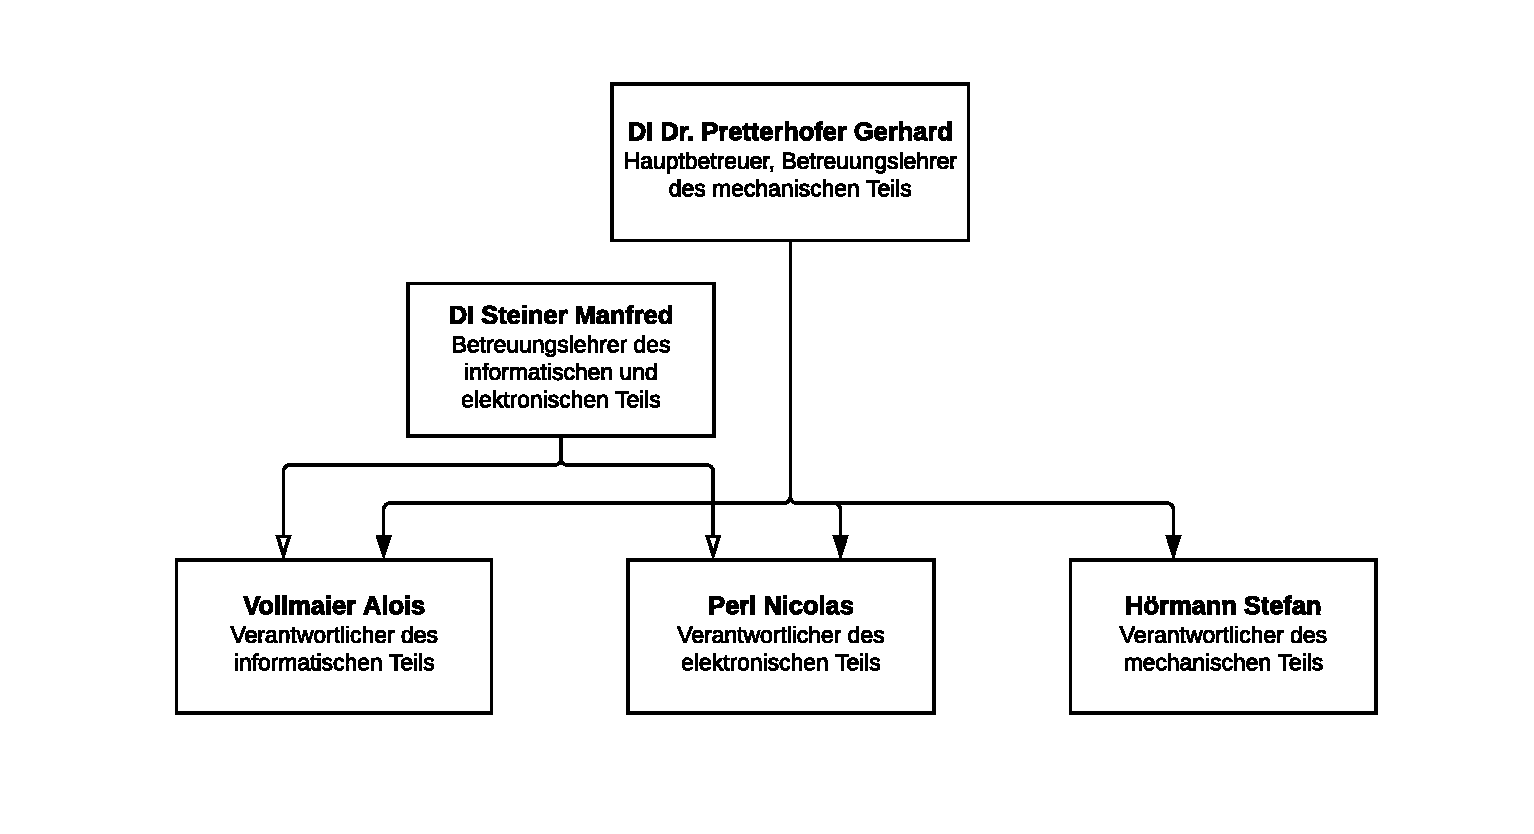
\includegraphics[width=0.80\textwidth]{fig/Hierachie_Reshuffled.pdf}
    \caption{Betreuerübersicht}
    \label{Bild über ganze Seitenbreite}
\end{figure}


\section{Konzept}
Wir setzten uns als Ziel eine Maschine zu entwickeln, welche das Mischen, sowie das Ausgeben von Spielkarten übernimmt.
Die Idee ist es, diese Verfahren möglichst platzsparend, zeiteffizient und detailliert durchdacht und optimiert zu realisieren.\\

\begin{wrapfigure}{r}{0.34\textwidth}
    \vspace{-40pt}
    \begin{center}
        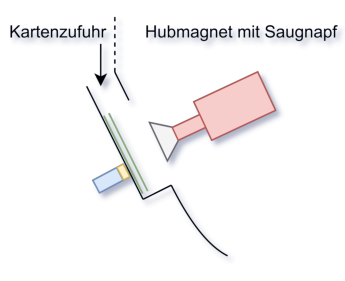
\includegraphics[width=0.35\textwidth]{fig/Reshuffled_Version_3_prinzip}
    \end{center}
    \caption{Kartenentnahme}
    \label{Kartenentnahme}
    \vspace{-15pt}
\end{wrapfigure}

Grundsätzlich basiert das Mischprinzip auf einer Art "Fächersystem".
Eingelegte Karten gelangen mithilfe eines ausgeklügelten Systems, welches aus einem Hubmagneten mit integriertem Saugnapf besteht, aus dem Einlegefach.
Erfolgt die Kartenentnahme, rutscht die Karte in ein zufälliges Fach des Lagerrads. Anschließend wird dieses Lagerrad in Drehbewegung versetzt um die gelagerten Karten auszugeben.

Der Benutzer steuert diese Maschiene auf einer GUI welche auf einem 7" LCD Display angezeigt wird. Systemintern steuert ein 8Bit Mikrocontroller der AVR-Familie den Ablauf.

%============================================
\chapter{Mechanik}
\lohead{Stefan Hörmann}
\label{sec:Mechanik}
\section{Beschreibung}

TODO


%============================================
\chapter{Elektronik}
\lohead{Nicolas Perl}
\label{sec:Elektronik}
\section{Beschreibung}

TODO



%============================================
\chapter{Informatik}
\lohead{Alois Vollmaier}
\label{sec:Informatik}
\section{Beschreibung}

Den Informatischen Teil der Arbeit kann man grundsätzlich in 2 Bereiche aufteilen. Einerseits soll eine einfache grafische Benutzeroberfläche gestaltet werden, auf welcher man den Mischvorgang steuern sowie grundlegende Einstellungen des Spieles vornehmen kann.
Aus programmtechnischen Gründen wird hierfür die Programmiersprache Java und das GUI-Toolkit Swing verwendet. \\
Die Hardwarekomponenten setzten sich aus einem Raspberry Pi 3B+ und einem 7" LCD Touchscreen der Firma Elecrow zusammen. \\

Andererseits besteht dieser Teilbereich der Arbeit auch aus der hardwarenahen Programmierung der Hauptplatine. Mithilfe der Programmiersprache C sollte der verbaute 8Bit Mikrocontroller der AVR-Familie namens ATmega 324P programmiert werden.
Dieser steuert den gesamten Ablauf der Maschiene. \\

Der Datenaustausch zwischen Hauptplatine und Raspberry PI erfolgt über die serielle Schnittstelle namens UART
{\itshape (Universal Asynchronous Receiver Transmitter)}
Hierfür wird die Open-Source-Bibliothek JSSC
{\itshape (Java Simple Serial Connector)}  verwendet.
%============================================
\chapter{Projektplanung}
\lohead{ReShuffled Projektplanung}
\label{sec:Projektplanung}
\section{Meilensteine}
\begin{table}[h!]
    \begin{tabular}{ll}
        \hline
        \rowcolor[HTML]{C0C0C0}
        \multicolumn{2}{c}{\cellcolor[HTML]{C0C0C0}\textbf{Meilensteine}}                      \\ \hline
        \rowcolor[HTML]{EFEFEF}
        \multicolumn{1}{l|}{\cellcolor[HTML]{EFEFEF}Datum} & Beschreibung                      \\ \hline
        \multicolumn{1}{l|}{15 Apr 2019}                   & Vollenden des Variantenvergleichs \\ \hline
        \multicolumn{1}{l|}{1 Jun 2019}                    & Fertigstellung der CAD Zeichnung  \\ \hline
        \multicolumn{1}{l|}{15 Sep 2019}                   & Fertigstellung der Hardware       \\ \hline
        \multicolumn{1}{l|}{31 Okt 2019}                   & Abschließen des Testaufbaus       \\ \hline
        \multicolumn{1}{l|}{1 Dez 2019}                    & Fertigstellung der Software       \\ \hline
    \end{tabular}
\end{table}

\section{Aufgabenplanung bis September}

Ziele des Herrn Hörmann:
\begin{itemize}
    \item Standartmäßig ist ein schwarzer Punkt davor.
    \item Die Länge ist nicht von Bedeutung, Zeilen werden automatisch umgebrochen.
\end{itemize}

\noindent\hrulefill

Ziele des Herrn Pearl:
\begin{itemize}
    \item Standartmäßig ist ein schwarzer Punkt davor.
    \item Die Länge ist nicht von Bedeutung, Zeilen werden automatisch umgebrochen.
\end{itemize}

\noindent\hrulefill

Ziele des Herrn Vollmaier:
\begin{itemize}
    \item Standartmäßig ist ein schwarzer Punkt davor.
    \item Die Länge ist nicht von Bedeutung, Zeilen werden automatisch umgebrochen.
\end{itemize}

%============================================
\chapter{Anhang}


\tikzset{isometricXYZ/.style={x={(-0.866cm,-0.5cm)}, y={(0.866cm,-0.5cm)}, z={(0cm,1cm)}}}
\tikzset{isometricZXY/.style={x={(0.866cm,-0.5cm)}, y={(0cm,1cm)}, z={(-0.866cm,-0.5cm)}}}
\tikzset{isometricYZX/.style={x={(0cm,1cm)}, y={(-0.866cm,-0.5cm)}, z={(0.866cm,-0.5cm)}}}
\begin{tikzpicture} [scale=4, isometricZXY, line join=round,
opacity=.75, text opacity=1.0,%
>=latex,
inner sep=0pt,%
outer sep=2pt,%
]

    \def\h{5}

    \newcommand{\quadrant}[2]{
    \foreach \t in {#1} \foreach \f in {175,165,...,5}
    \draw [fill=#2]
    ({sin(\f - \h)*cos(\t - \h)}, {sin(\f - \h)*sin(\t - \h)}, {cos(\f - \h)})
    -- ({sin(\f - \h)*cos(\t + \h)}, {sin(\f - \h)*sin(\t + \h)}, {cos(\f - \h)})
    -- ({sin(\f + \h)*cos(\t + \h)}, {sin(\f + \h)*sin(\t + \h)}, {cos(\f + \h)})
    -- ({sin(\f + \h)*cos(\t - \h)}, {sin(\f + \h)*sin(\t - \h)}, {cos(\f + \h)})
    -- cycle;
    }

    %Quadrants
    \quadrant{220,230,...,300}{black}
    \quadrant{-60,-50,...,20}{white}
    \quadrant{30,40,...,120}{black}
    \quadrant{130,140,...,210}{none}

    %Movement arrows
    \foreach \t in {225,235,...,295}
    \foreach \f in {50,40,...,0}
    \draw [red, opacity=1.0, ->, thick]
    ({sin(\f - \h)*cos(\t - \h)}, {sin(\f - \h)*sin(\t - \h)}, {cos(\f - \h)})
    -- ({(1 + 0.2*cos(90 - \f))*sin(\f - \h)*cos(\t - \h)},
    {(1 + 0.2*cos(90 - \f))*sin(\f - \h)*sin(\t - \h)},
    {(1 + 0.2*cos(90 - \f))*cos(\f - \h)});

    \foreach \t in {125,135,...,205}
    \foreach \f in {110,100,...,0}
    \draw [black, ->, thick]
    ({(1 + 0.2*cos(90 - \f))*sin(\f - \h)*cos(\t - \h)},
    {(1 + 0.2*cos(90 - \f))*sin(\f - \h)*sin(\t - \h)},
    {(1 + 0.2*cos(90 - \f))*cos(\f - \h)})
    -- ({sin(\f - \h)*cos(\t - \h)},{sin(\f - \h)*sin(\t - \h)},{cos(\f - \h)});
    \foreach \t in {35,45,...,115}
    \foreach \f in {130,120,...,0}
    \draw [red, opacity=1.0 ,->, thick]
    ({sin(\f - \h)*cos(\t - \h)}, {sin(\f - \h)*sin(\t - \h)}, {cos(\f - \h)})
    -- ({(1 + 0.2*cos(90 - \f))*sin(\f - \h)*cos(\t - \h)},
    {(1 + 0.2*cos(90 - \f))*sin(\f - \h)*sin(\t - \h)},
    {(1 + 0.2*cos(90 - \f))*cos(\f - \h)});

    \foreach \t in {-55,-45,...,25}
    \foreach \f in {130,120,...,0}
    \draw [black, ->, thick]
    ({(1 + 0.2*cos(90 - \f))*sin(\f - \h)*cos(\t - \h)},
    {(1 + 0.2*cos(90 - \f))*sin(\f - \h)*sin(\t - \h)},
    {(1 + 0.2*cos(90 - \f))*cos(\f - \h)})
    -- ({sin(\f - \h)*cos(\t - \h)},{sin(\f - \h)*sin(\t - \h)},{cos(\f - \h)});

    %Annotations
    \path ({1.5*sin(100)*cos(75)}, {1.5*sin(100)*sin(75)}, {1.5*cos(100)}) node [right] {Compression};
    \path ({1.5*sin(70)*cos(-15)}, {1.5*sin(70)*sin(-15)}, {1.5*cos(70)})  node [right] {Dilatation};
    \path ({1.25*sin(50)*cos(165)},{1.25*sin(50)*sin(165)},{1.25*cos(50)}) node [left]  {Dilatation};
    \path ({1.25*sin(30)*cos(255)},{1.25*sin(30)*sin(255)},{1.25*cos(30)}) node [left]  {Compression};

    %P and T axis
    \begin{scope}[ultra thick]
        \draw[->] ({1.75*sin(90)*cos(75)}, {1.75*sin(90)*sin(75)}, {1.75*cos(90)})
        -- ({2*sin(90)*cos(75)},{2*sin(90)*sin(75)},{2*cos(90)}) node [above] {T-axis};
        \draw[->] ({1.75*sin(90)*cos(255)},{1.75*sin(90)*sin(255)},{1.75*cos(90)})
        -- ({2*sin(90)*cos(255)},{2*sin(90)*sin(255)},{2*cos(90)}) node [below] {T-axis};
        \draw[<-] ({1.5*sin(90)*cos(-15)}, {1.5*sin(90)*sin(-15)}, {1.5*cos(90)})
        -- ({1.75*sin(90)*cos(-15)},{1.75*sin(90)*sin(-15)},{1.75*cos(90)}) node [right] {P-axis};
        \draw[<-] ({1.5*sin(90)*cos(165)}, {1.5*sin(90)*sin(165)}, {1.5*cos(90)})
        -- ({1.75*sin(90)*cos(165)},{1.75*sin(90)*sin(165)},{1.75*cos(90)}) node [left] {P-axis};
    \end{scope}

    % Label
    \node [anchor=north, yshift=-2mm] at (current bounding box.south)
    {Seismic focal mechanism and Pression-Tension axis.};
\end{tikzpicture}

													% Datei importieren


\renewcommand\appendixname{Anhang}
\renewcommand\appendixpagename{Anhang}
\renewcommand\appendixtocname{Anhang}

\lohead{}

% Anhang Seite ohne Kopf- & Fußzeile
\appendix
\begingroup
\makeatletter
\let\ps@plain\ps@empty
\appendixpage
\makeatother
\endgroup

% Anhänge
\chapter{Zeitaufzeichnung}
\chapter{Persönlicher Anhang 1}

\markboth{}{}	%end chapter

\printbibliography
\nocite{*}

\chapter{Abkürzungsverzeichnis}
\begin{acronym}
	%Abkürzung hinzufügen: \acro{Kürzel}{Ausgeschrieben}
	\acro{WLAN}{Wireless Local Area Network}
	\acro{WWW}{World Wide Web}
	\acro{uC}[µC]{Mikrocontroller}
\end{acronym}

\listoffigures
\listoftables
\lstlistoflistings													% Datei importieren
\end{document}
